\documentclass{beamer}
\usepackage{graphicx}
\usepackage[english,activeacute]{babel}
\usepackage[utf8]{inputenc}
\usepackage{color}
\usepackage{tikz}

\usetheme[pageofpages=of,
          alternativetitlepage=true,
          titlepagelogo=,%img/src/lirae,
          watermark=,%img/src/lirae-off,
          watermarkheight=80px,
          watermarkheightmult=1,
          ]{Torino}

%\titlegraphic{
%   \hspace{-5cm}
%   
\includegraphics[height=1cm]{img/src/csrg}
%   \hfill
%   
\includegraphics[height=1cm]{img/src/utfsm}
%   %\hfill
%   %
\includegraphics[height=1.2cm]{img/src/lirae}
%}

\usecolortheme{lirae}

%title%
\title[Short title]{\huge{Chilean Virtual Observatory}}
\author{Mauricio Solar \\
        % email
        \small{\textcolor{gray}{\texttt{msolar@inf.utfsm.cl}}}}
\institute[CSRG-UTFSM]{
%Computer Systems Research Group,\\
Universidad Técnica Fedrico Santa María
}
\date{\today}


\begin{document}

%first slide%
\begin{frame}[t,plain]
\titlepage
\end{frame}



\begin{frame}
	\frametitle{Overview}
	\tableofcontents
\end{frame}

\section{Who am I, and how did I get here?}

\begin{frame}
\frametitle{Who am I?}
\begin{itemize}
	\item Mauricio Solar Fuentes, Ph.D in Computer Sciences, expertise in artificial intelligence, parallel computing.
	\item Director of project entitled: "Development of an Astro-Informatic Platform for Management and 
		Intelligent Analysis of Large-scale Data".
	\item I come representing the Chilean Community, which is now working to create the Chilean Virtual Observatory.
\end{itemize}
\end{frame}

\section{Motivation}

\begin{frame}
\frametitle{Motivation}

\begin{itemize}
	\item In Chile, the astronomy has become one of the scientific fields with a surprising growth rate in the last years.
	\item There are more than a dozen astronomical facilities in our country, for example:
		\begin{enumerate}
			\addtolength{\itemindent}{1cm}
			\item Atacama Large Millimeter/submillimeter Array (ALMA)
			\item Very Large Telescope (VLT)
			\item And soon the European Extremely Large Telescope (E-ELT)
		\end{enumerate}
	\item One of the conditions established in our country, is that the 10\% of the observation
		time belongs to the Chilean astronomical community
	\item \emph{\textbf{Motivation}}: it's necessary to develop an astroinformatic platform for the data administration 
		and intelligent analysis.
\end{itemize}

\end{frame}

% Split in several slides and add a diagram or photo
\section{Goals}

\begin{frame}
\frametitle{Considered issues}

The ALMA project, which when fully operational will generate over 1TB of data per observation day. So, we consider the
following issues:

\begin{itemize}
	\item \textbf{Storage}, is necessary to have data center capable of storage according the data consumption needs.
\end{itemize}

\begin{center}
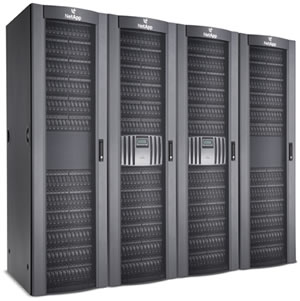
\includegraphics[height=0.3\textheight]{img/storage}
\end{center}

\end{frame}


\begin{frame}
\frametitle{Considered issues}
\begin{itemize}
	\item \textbf{Access}, in this project it has been decided that a web system is an appropriate mechanism to supply
		this requirement.
\end{itemize}

\begin{center}

\includegraphics[height=0.3\textheight]{img/access}
\end{center}

\end{frame}


\begin{frame}
\frametitle{Considered issues}
\begin{itemize}
	\item \textbf{Processing}: Having large volumes of data, the processing to accomplish, requires more time than usual
		and computational resources. So a computational cluster, can be an useful tool to facilitate this work.
\end{itemize}

\begin{center}

\includegraphics[height=0.3\textheight]{img/processing}
\end{center}

\end{frame}

%Comunidad
%
%Actualmente se está desarrollando el proyecto titulado “Desarrollo de una
%plataforma astroinformática para la administración y análisis de datos de gran
%escala”, financiado por fondos gubernamentales (FONDEF D11I1060), con duración
%de 28 meses, en el cual participan las siguientes instituciones:
%
%- Atacama Large Milimiter/submilimiter Array
%
%- Consorcio Red Universitaria Nacional Reuna
%
%- Universidad Técnica Federico Santa María
%
%- Universidad de Chile
%
%- Universidad Católica de Chile
%
%- Universidad de Concepción
%
%- Universidad de Santiago de Chile
%
%Los objetivos del proyecto están relacionados con el diseño e implementación de
%un observatorio virtual, el cual deberá cumplir con los estándares de la
%“International Virtual Observatory Alliance” (IVOA). Además los astrónomos
%investigadores del proyecto, crearán instancias donde presentarán problemáticas
%que enfrentan como comunidad, ante el procesamiento de datos, los cuales se
%resolverán mediante técnicas computacionales conocidas por los investigadores
%del área de computación.
%
%El presente proyecto se realiza en estrecha colaboración con ALMA, quienes
%aportan su visión desde el punto de vista de observatorio, comparten
%conocimiento respecto a los modelos y tipos de datos que se usan, y además se
%establecerán políticas de colaboración para facilitar el acceso a los datos.
%
%Por otro lado el Consorcio Red Universitaria Nacional Reuna y el
%National Laboratory for High Performance Computing juega otro rol
%importante, ya que una de las problemáticas a resolver es la conectividad de
%altas tasas de transmisión de datos (REUNA) y almacenar datos que exigen
%grandes capacidades de almacenamiento (NLHPC).
%
%En conjunto estas instituciones unen esfuerzos para lograr crear y establecer
%en el tiempo una plataforma sin precedente en el área astroinformática Chilena,
%el Chilean Virtual Observatory (ChiVO http://www.chivo.cl/).

\section{Involved community}

Currently, a project entitled "Development of an Astro-Informatic Platform
for Management and Intelligent Analysis of Large-scale Data" is being developed,
financed by government funding (FONDEF D11I1060), for a period of 28 months,
and with the participation of the following institutions:

\begin{itemize}
	\item Atacama Large Milimiter/submilimiter Array (ALMA)
	\item Consorcio Red Universitaria Nacional Reuna (REUNA)
	\item Universidad Técnica Federico Santa María
	\item Universidad de Chile
	\item Universidad Católica de Chile
	\item Universidad de Concepción
	\item Universidad de Santiago de Chile
\end{itemize}

The goals of the project are related to the design and implementation of a
virtual observatory, which shall comply the standars of the International
Virtual Observatory Allience (IVOA). In addition the astronomers of the
project will create instances where they will present problems faced as a community,
related to data processin, which will be solved by computational techniques
known by the researchers in the computing field.

This project is conducted in close collaboration with ALMA who bring their
vision from the point of view of an observatroy, sharing their knowledge about models and
used data types, and also establishing collaborative policies to
facilitate the access to data.

On the other hand, the "Consorcio Red Universitaria Nacional" and the National
Laboratory for High Performance Computing, plays another important role, as the solution
of the problem related to the connectivity of high rate data transmission
(REUNA) and storing the data will require large storage capabilities (NLHPC).

These institutions join efforts to achieve, create and establish in
time a platform unprecedented in the chilean astroinformatics field, the Chilean
Virtual Observatory (ChiVO).




%final slide%
\begin{frame}[t,plain]
\titlepage
\end{frame}
\end{document}
